\documentclass[conference]{IEEEtran}
\IEEEoverridecommandlockouts
% The preceding line is only needed to identify funding in the first footnote. If that is unneeded, please comment it out.
\usepackage{cite}
\usepackage{amsmath,amssymb,amsfonts}
\usepackage{algorithmic}
\usepackage{graphicx}
\graphicspath{{figures/}}
\usepackage{textcomp}
\usepackage{xcolor}
\usepackage{balance}
\def\BibTeX{{\rm B\kern-.05em{\sc i\kern-.025em b}\kern-.08em
    T\kern-.1667em\lower.7ex\hbox{E}\kern-.125emX}}
\begin{document}

\title{Conference Paper Title}


\author{\IEEEauthorblockN{Luca Schumann}
\IEEEauthorblockA{\textit{lucsc442} \\
\textit{TDDE16}}
}

\maketitle

\begin{abstract}
Test
\end{abstract}

\section{Introduction}
Introduce the task or research question that you have addressed in
your project. What were you trying to do? Why did you choose this project?

\section{Theory}
Present relevant theoretical background, and in particular the models that
you have used. Where appropriate, use mathematical formulas.

\section{Data}
Present your data. What information does it contain? Where did you get it
from? What preprocessing did you do, if any?

\subsection{Dataset}
First of all, a selection of songs had to be made. To find a balance between relevant artists in the CD era and the streaming era, I decided to combine lists of artists from two sources. I selected all 46 german artists from the Wikipedia list of Rappers that sold more than 100,000 albums in Germany \cite{wiki_albums}. The popularity of musicians today, especially Rappers, is not only defined by the albums sales but also the online streams. Therefore I picked all 13 Rappers appearing in the Spotify playlist "Top German Artists of 2020" \cite{spotify_2020} that were not in the selection yet. To increase the dataset, I chose 18 more objectively popular Rappers, adding up to 77 artists in the end.\\
The lyrics of the artists' songs were then downloaded using the Genius API \cite{genius} with help of the \textit{lyricsgenius}package \cite{lyricsgenius}. A lot of the songs are duplicates, since remixes, features and live versions are all included in the genius database. There are furthermore many non-songs in the database, such as commentaries. Luckily, most could easily be ignored by discarding songs that contain brackets, as in \textit{Papa ist da (AsadJohn Remix)}. Few others had to be handled differently, but the final dataset is clean of such occurences. In a first run of the model, songs containing english lyrics formed an individual topic. Upon manual inspection, there were a few songs with parts in english, or even completely in english. Therefore, songs that contain all the most common english words in the english topic "the", "you" and "and" were suspected to contain english lyrics and also discarded. The final dataset features almost 7500 songs.

\subsection{Preprocessing}
Preprocessing the song lyrics was an iterative process with many learned lessons. The most basic first step is to remove meta information that is written in brackets from the lyrics, such as \textit{[Hook]}. Next, the songs are tokenized using spacy's German package. Non-alphabetic tokens, stop words and tokens with less than three letters are removed. The rest of the preprocessing is done with Gensim. Bigrams and Trigrams are added and extremes are filtered. Finding the seemingly best values for these tasks was done with the trial and error method.\\
After excluding english songs from the dataset, the model would still find a topic with mostly english stop words. After removing english stop words during preprocessing, the problem was solved. Another problem was many artist's names appearing in the most salient words of some topics. The reason for this is that some Rappers are notorious for talking and singing about themselves in the third person. Rappers with a lot of songs in the dataset would therefore skew the results, although their own name has nothing to do with the message behind their song. To tackle the problem, each artists name was removed from his or her lyrics. As a final tweak of the preprocessing step, a couple of stop words that were not in spacy's German list were manually removed.\\
Tokenizing German text turned out to be a difficult task, with no really satisfying solution. In German texts, all nouns are capitalized, therefore also in spacy's word list. If a word at the beginning of a sentence is capitalized, it is not possible for spacy to tell wether it's a noun or not. Feeding spacy all words in lowercase would also not solve the problem, since it would not recognize the nouns anymore. Additionally, some words have a different meaning depending on wether they are a noun (capitalized) or not. E.g. "Weg" means path but "weg" means away in German. This appears to be an unsolved problem as of today, as can be read on spacy's Github forum \cite{spacy_issues}. Lemmatization does also not work as well as for english text, but overall the results are good enough to work with them.

\section{Method}
Explain how you carried out your study. Aim to be detailed enough for
others to reproduce your results.

\section{Results}
Present your results in an objective way. Use tables and charts, but do not
forget to also include a summary in text form. Do not interpret your results

\subsection{Topics in Rap over Time}
In this section I visualize the development of German Hip Hop lyrics over the last 30 years. Figure \ref{fig:timeline} depicts the average topic distribution of all songs that were released in the respective year. Since the number of songs released differs each year, the data is normalized to better capture the bigger picture. Note that they years until 2003 contain less than 100 songs each, whereas each year after 2011 has more than 400 songs in the dataset. This imbalance is not due to a poorly select subset of artists, but rather due to the rapid growth in popularity of German Rap in the last 10 years \cite{musikindustrie}. Multiple trends can be seen in this graphic. First of all, an increase of the topic "Competition" with a peak in 2005, followed by a steady decline until 2018. Next, we observe a fast growth of the "Lifestyle" topic since 2010, as well as a moderate growth of "Street" Rap between 2008 and 2018. Throughout most years, "Love \& Life" appears to be the most dominant topic.\\
This method automatically gives higher influence to artists with more songs in a release year. It also disregards the music preferences of the audience. Figure \ref{fig:w_timeline} is meant to capture the preferred topics by the consumers, by weighting each song with its Spotify popularity score. The score is downloaded for each song from the Spotify API using the \textit{spotipy} package \cite{spotipy}. It measures the current popularity of a song on a scale from 0 to 100. To increase the influence of more popular songs on the graphic, I extended the scale to 1000. An exponential function maps e.g. the score 100 to 1000 or 90 to ca. 500. Compared to the unweighted graphic, we immediately notice a much higher share of the topics "Street" and "Sex \& Party" throughout the entire timeline. The topics "Love \& Life" and "Competition" on the other hand seem to be less popular. "Lifestyle" is mostly unchanged by the weighting.

\begin{figure}[!t]
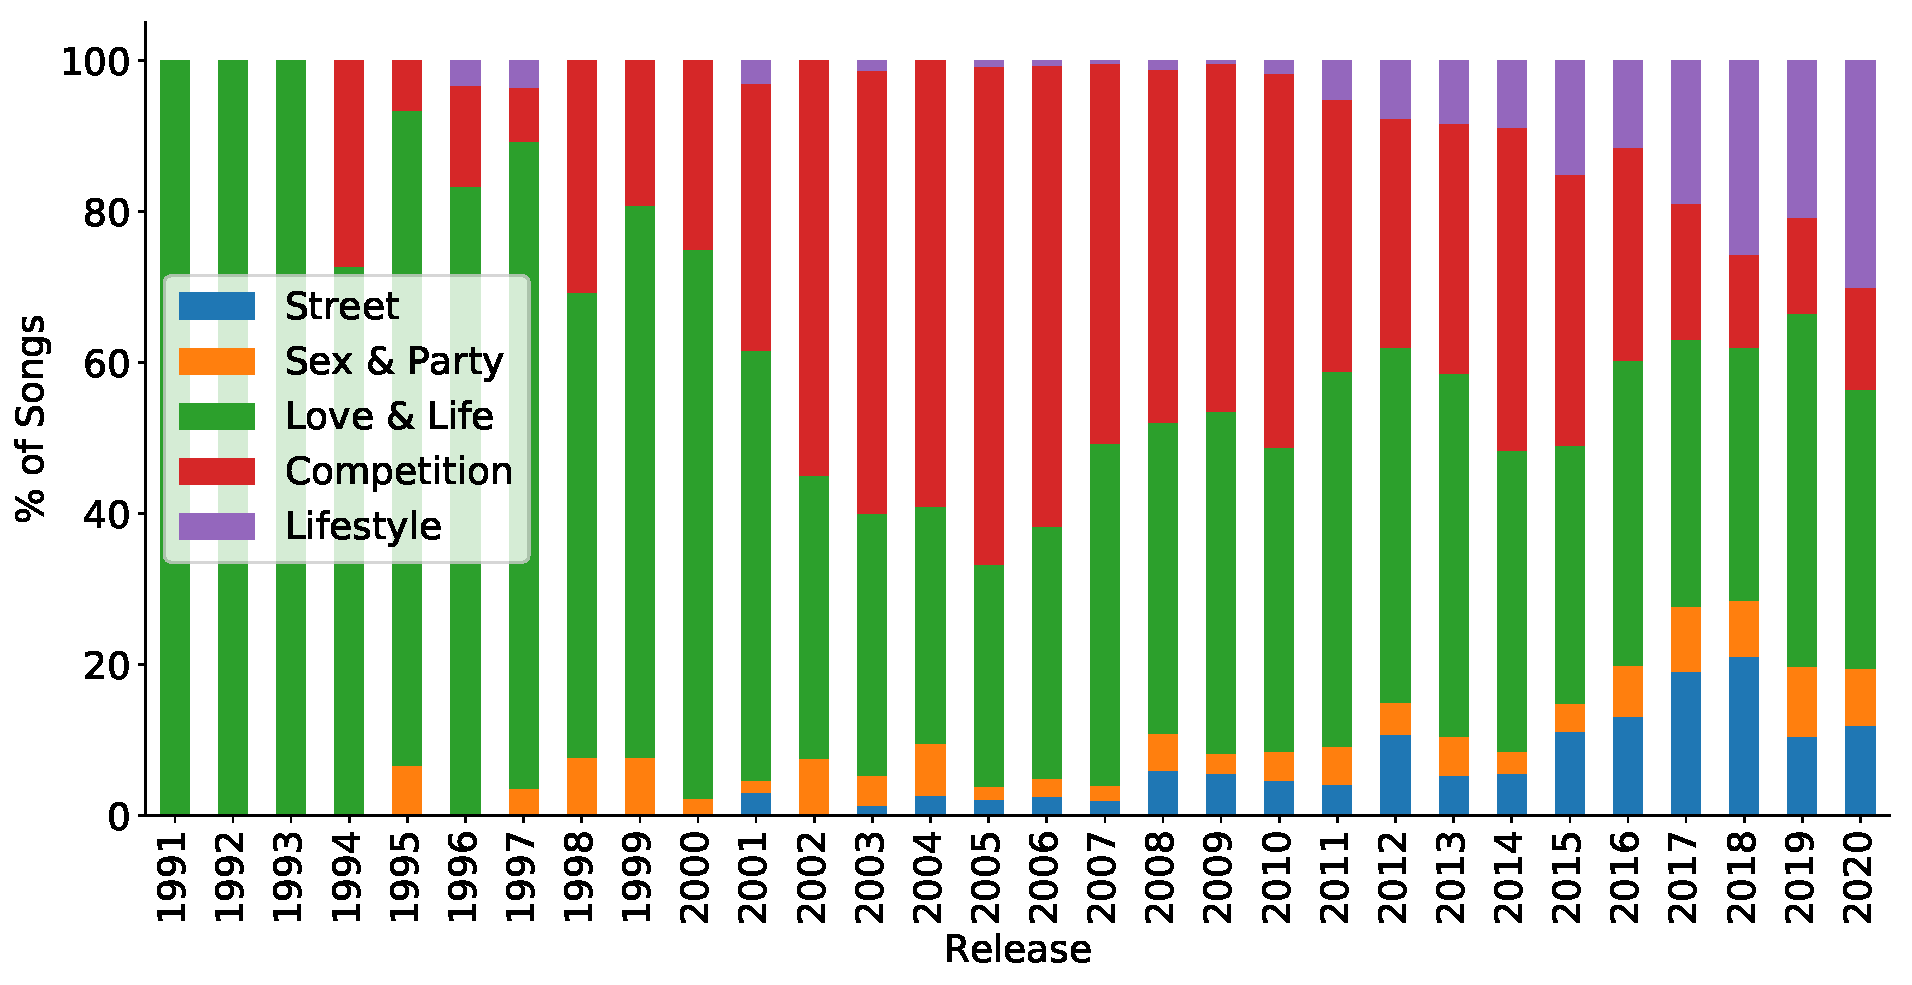
\includegraphics[width=\linewidth]{figures/timeline.pdf}
\vspace*{-8mm}
\caption{Normalized timeline of the average topic distribution in the lyrics of songs released between 1991 and 2020.}
\label{fig:timeline}
\end{figure}

\begin{figure}[!t]
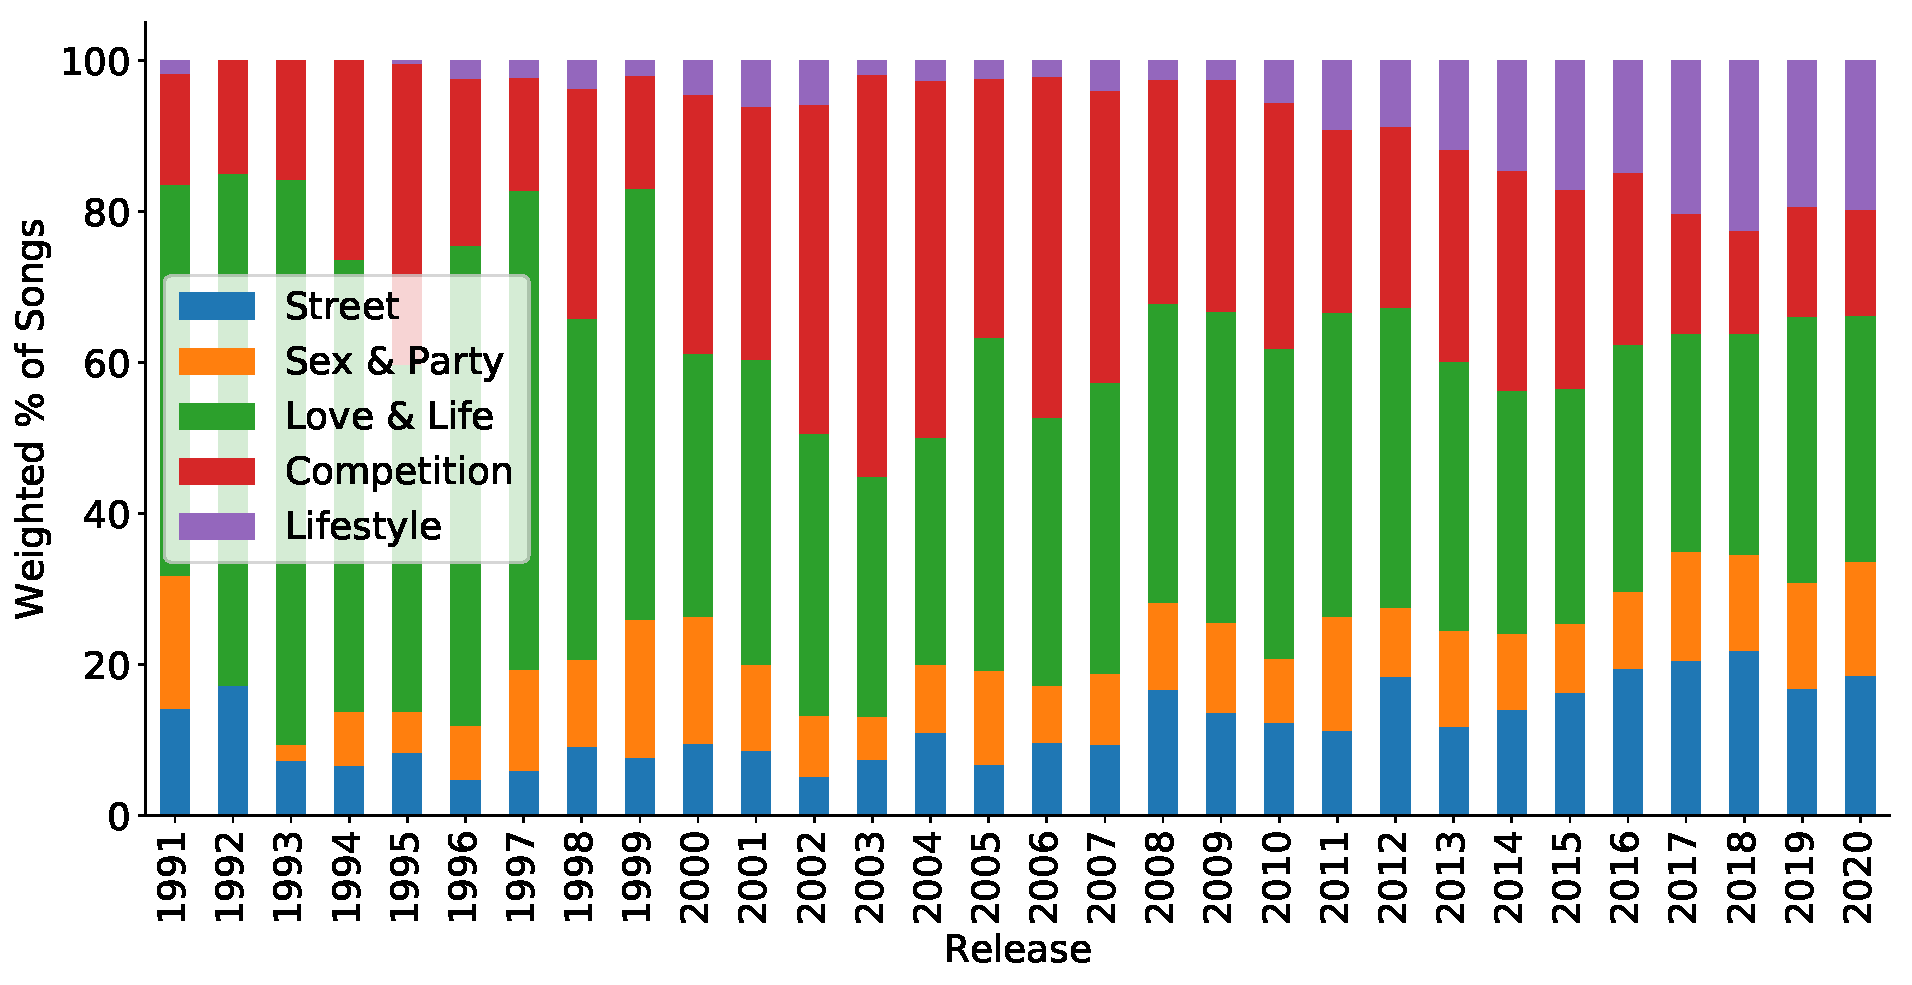
\includegraphics[width=\linewidth]{figures/w_timeline.pdf}
\vspace*{-8mm}
\caption{Normalized timeline of the average topic distribution in the lyrics of songs released between 1991 and 2020. Songs are weighted by their popularity score on Spotify.}
\label{fig:w_timeline}
\end{figure}

\subsection{name?}
\subsection{Sido's Story - Underground to Mainstream}


\section{Discussion}
Analyse your results and discuss the possibilities and limitations of
your technical approach. Compare your study to related work.

\section{Conclusion}
Based on your results and their analysis, what new knowledge do you
take away from your project?

\section{TODOBELOW}

\subsection{Abbreviations and Acronyms}\label{AA}

\subsection{Units}
\begin{itemize}
\item Use either SI (MKS) or CGS as primary units. (SI units are encouraged.) English units may be used as secondary units (in parentheses). An exception would be the use of English units as identifiers in trade, such as ``3.5-inch disk drive''.
\item Avoid combining SI and CGS units, such as current in amperes and magnetic field in oersteds. This often leads to confusion because equations do not balance dimensionally. If you must use mixed units, clearly state the units for each quantity that you use in an equation.
\item Do not mix complete spellings and abbreviations of units: ``Wb/m\textsuperscript{2}'' or ``webers per square meter'', not ``webers/m\textsuperscript{2}''. Spell out units when they appear in text: ``. . . a few henries'', not ``. . . a few H''.
\item Use a zero before decimal points: ``0.25'', not ``.25''. Use ``cm\textsuperscript{3}'', not ``cc''.)
\end{itemize}

\subsection{Equations}
Number equations consecutively. To make your 
equations more compact, you may use the solidus (~/~), the exp function, or 
appropriate exponents. Italicize Roman symbols for quantities and variables, 
but not Greek symbols. Use a long dash rather than a hyphen for a minus 
sign. Punctuate equations with commas or periods when they are part of a 
sentence, as in:
\begin{equation}
a+b=\gamma\label{eq}
\end{equation}

Be sure that the 
symbols in your equation have been defined before or immediately following 
the equation. Use ``\eqref{eq}'', not ``Eq.~\eqref{eq}'' or ``equation \eqref{eq}'', except at 
the beginning of a sentence: ``Equation \eqref{eq} is . . .''

\subsection{\LaTeX-Specific Advice}

Please use ``soft'' (e.g., \verb|\eqref{Eq}|) cross references instead
of ``hard'' references (e.g., \verb|(1)|). That will make it possible
to combine sections, add equations, or change the order of figures or
citations without having to go through the file line by line.

Please don't use the \verb|{eqnarray}| equation environment. Use
\verb|{align}| or \verb|{IEEEeqnarray}| instead. The \verb|{eqnarray}|
environment leaves unsightly spaces around relation symbols.

Please note that the \verb|{subequations}| environment in {\LaTeX}
will increment the main equation counter even when there are no
equation numbers displayed. If you forget that, you might write an
article in which the equation numbers skip from (17) to (20), causing
the copy editors to wonder if you've discovered a new method of
counting.

{\BibTeX} does not work by magic. It doesn't get the bibliographic
data from thin air but from .bib files. If you use {\BibTeX} to produce a
bibliography you must send the .bib files. 

{\LaTeX} can't read your mind. If you assign the same label to a
subsubsection and a table, you might find that Table I has been cross
referenced as Table IV-B3. 

{\LaTeX} does not have precognitive abilities. If you put a
\verb|\label| command before the command that updates the counter it's
supposed to be using, the label will pick up the last counter to be
cross referenced instead. In particular, a \verb|\label| command
should not go before the caption of a figure or a table.

Do not use \verb|\nonumber| inside the \verb|{array}| environment. It
will not stop equation numbers inside \verb|{array}| (there won't be
any anyway) and it might stop a wanted equation number in the
surrounding equation.

\subsection{Some Common Mistakes}\label{SCM}
\begin{itemize}
\item The word ``data'' is plural, not singular.
\item The subscript for the permeability of vacuum $\mu_{0}$, and other common scientific constants, is zero with subscript formatting, not a lowercase letter ``o''.
\item In American English, commas, semicolons, periods, question and exclamation marks are located within quotation marks only when a complete thought or name is cited, such as a title or full quotation. When quotation marks are used, instead of a bold or italic typeface, to highlight a word or phrase, punctuation should appear outside of the quotation marks. A parenthetical phrase or statement at the end of a sentence is punctuated outside of the closing parenthesis (like this). (A parenthetical sentence is punctuated within the parentheses.)
\item A graph within a graph is an ``inset'', not an ``insert''. The word alternatively is preferred to the word ``alternately'' (unless you really mean something that alternates).
\item Do not use the word ``essentially'' to mean ``approximately'' or ``effectively''.
\item In your paper title, if the words ``that uses'' can accurately replace the word ``using'', capitalize the ``u''; if not, keep using lower-cased.
\item Be aware of the different meanings of the homophones ``affect'' and ``effect'', ``complement'' and ``compliment'', ``discreet'' and ``discrete'', ``principal'' and ``principle''.
\item Do not confuse ``imply'' and ``infer''.
\item The prefix ``non'' is not a word; it should be joined to the word it modifies, usually without a hyphen.
\item There is no period after the ``et'' in the Latin abbreviation ``et al.''.
\item The abbreviation ``i.e.'' means ``that is'', and the abbreviation ``e.g.'' means ``for example'' \cite{genius}.
\end{itemize}

\subsection{Authors and Affiliations}
\textbf{The class file is designed for, but not limited to, six authors.} A 
minimum of one author is required for all conference articles. Author names 
should be listed starting from left to right and then moving down to the 
next line. This is the author sequence that will be used in future citations 
and by indexing services. Names should not be listed in columns nor group by 
affiliation. Please keep your affiliations as succinct as possible (for 
example, do not differentiate among departments of the same organization).

\subsection{Identify the Headings}
Headings, or heads, are organizational devices that guide the reader through 
your paper. There are two types: component heads and text heads.

Component heads identify the different components of your paper and are not 
topically subordinate to each other. Examples include Acknowledgments and 
References and, for these, the correct style to use is ``Heading 5''. Use 
``figure caption'' for your Figure captions, and ``table head'' for your 
table title. Run-in heads, such as ``Abstract'', will require you to apply a 
style (in this case, italic) in addition to the style provided by the drop 
down menu to differentiate the head from the text.

Text heads organize the topics on a relational, hierarchical basis. For 
example, the paper title is the primary text head because all subsequent 
material relates and elaborates on this one topic. If there are two or more 
sub-topics, the next level head (uppercase Roman numerals) should be used 
and, conversely, if there are not at least two sub-topics, then no subheads 
should be introduced.

\subsection{Figures and Tables}
\paragraph{Positioning Figures and Tables} Place figures and tables at the top and 
bottom of columns. Avoid placing them in the middle of columns. Large 
figures and tables may span across both columns. Figure captions should be 
below the figures; table heads should appear above the tables. Insert 
figures and tables after they are cited in the text. Use the abbreviation 
``Fig.~\ref{fig}'', even at the beginning of a sentence.

\begin{table}[htbp]
\caption{Table Type Styles}
\begin{center}
\begin{tabular}{|c|c|c|c|}
\hline
\textbf{Table}&\multicolumn{3}{|c|}{\textbf{Table Column Head}} \\
\cline{2-4} 
\textbf{Head} & \textbf{\textit{Table column subhead}}& \textbf{\textit{Subhead}}& \textbf{\textit{Subhead}} \\
\hline
copy& More table copy$^{\mathrm{a}}$& &  \\
\hline
\multicolumn{4}{l}{$^{\mathrm{a}}$Sample of a Table footnote.}
\end{tabular}
\label{tab1}
\end{center}
\end{table}

\begin{figure}[htbp]
\centerline{
\includegraphics{fig1.png}}
\caption{Example of a figure caption.}
\label{fig}
\end{figure}

Figure Labels: Use 8 point Times New Roman for Figure labels. Use words 
rather than symbols or abbreviations when writing Figure axis labels to 
avoid confusing the reader. As an example, write the quantity 
``Magnetization'', or ``Magnetization, M'', not just ``M''. If including 
units in the label, present them within parentheses. Do not label axes only 
with units. In the example, write ``Magnetization (A/m)'' or ``Magnetization 
\{A[m(1)]\}'', not just ``A/m''. Do not label axes with a ratio of 
quantities and units. For example, write ``Temperature (K)'', not 
``Temperature/K''.

\section*{References}

Please number citations consecutively within brackets. The 
sentence punctuation follows the bracket.

{
\balance{
  \bibliographystyle{IEEEtran}
  \bibliography{report.bib}
  }
}
\end{document}
